\section{ПО для настройки БПЛА}

Прошивка полётного контроллера определяет, что умеет дрон. Три главных открытых проекта: \textbf{Betaflight}, \textbf{INAV} и \textbf{ArduPilot} (плюс PX4). Настройка выполняется через программу-\term{конфигуратор} или \term{наземную станцию} (GCS), подключённую по USB или по радио.

\begin{figure}[H]\centering
\begin{tikzpicture}[font=\sffamily\small,node distance=4mm]
\node[blk,fill=gray!15] (mw) {MultiWii (2010)};
\node[blk,fill=gray!15,right=of mw] (bf0) {Baseflight};
\node[blk,fill=gray!15,right=of bf0] (cf) {Cleanflight};
\node[blk,fill=blk4,above right=2mm and 6mm of cf] (bf) {\textbf{Betaflight}};
\node[blk,fill=blk2,below right=2mm and 6mm of cf] (inav) {\textbf{INAV}};
\draw[arr] (mw) -- (bf0); \draw[arr] (bf0) -- (cf); \draw[arr] (cf.east) -- (bf.west); \draw[arr] (cf.east) -- (inav.west);
\node[blk,fill=blk1,below=10mm of mw,xshift=12mm] (ap) {\textbf{ArduPilot} (с 2009, APM $\to$ Pixhawk)};
\node[blk,fill=blk1,right=of ap] (px4) {PX4 (ETH Zürich)};
\end{tikzpicture}
\caption{«Родословная» прошивок}
\end{figure}

\subsection{Betaflight}
\begin{itemize}
\item \textbf{Назначение}: FPV-мультикоптеры — гонки, фристайл, синематик. Лучшая «ручная» управляемость.
\item Основной режим — \term{Acro} (Rate): стики задают \emph{угловую скорость}, самовыравнивания нет. Есть Angle/Horizon (с самовыравниванием), \textbf{GPS Rescue} (аварийный возврат), но нет полётов по точкам.
\item Программа: \textbf{Betaflight Configurator} (сейчас — веб-приложение \url{app.betaflight.com}).
\item Основные вкладки: \textbf{Setup} (калибровка акселерометра, 3D-модель), \textbf{Ports} (назначение UART), \textbf{Configuration} (тип рамы, протокол ESC, датчики), \textbf{Power \& Battery}, \textbf{Failsafe}, \textbf{PID Tuning} (ПИД, фильтры, рейты), \textbf{Receiver} (протокол, проверка каналов), \textbf{Modes} (ARM, режимы на тумблерах AUX), \textbf{Motors} (проверка моторов, направление), \textbf{OSD}, \textbf{Video Transmitter}, \textbf{Blackbox}, \textbf{CLI} (командная строка: \code{diff all}, \code{set}, \code{save}), \textbf{Presets} (готовые настройки).
\item Особенности: RPM-фильтр (по данным двунаправленного DShot), динамические фильтры, Blackbox-логи для настройки ПИД.
\end{itemize}

\begin{figure}[H]\centering
\begin{subfigure}[b]{0.49\linewidth}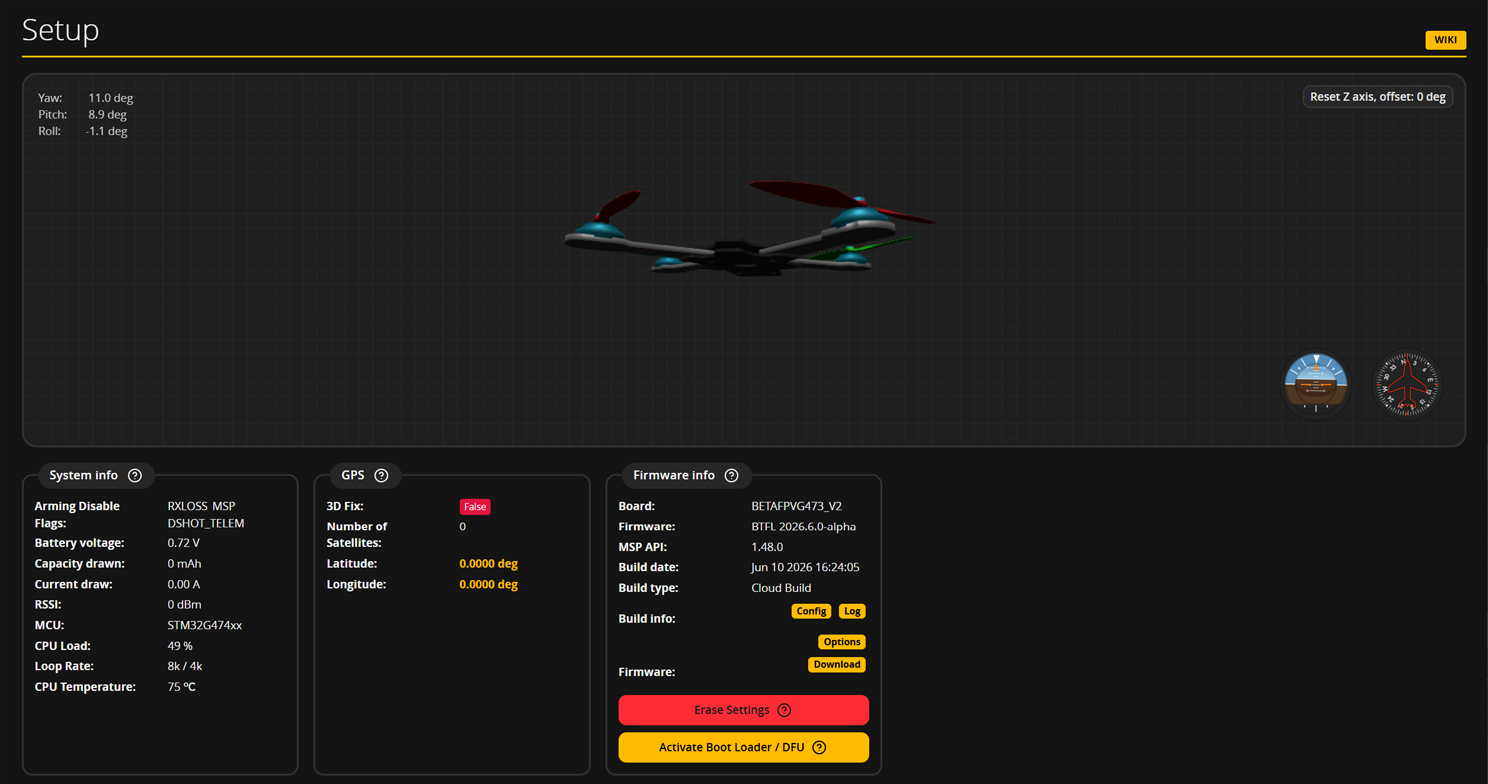
\includegraphics[width=\linewidth]{img/bf-setup.png}\caption{Setup}\end{subfigure}\hfill
\begin{subfigure}[b]{0.49\linewidth}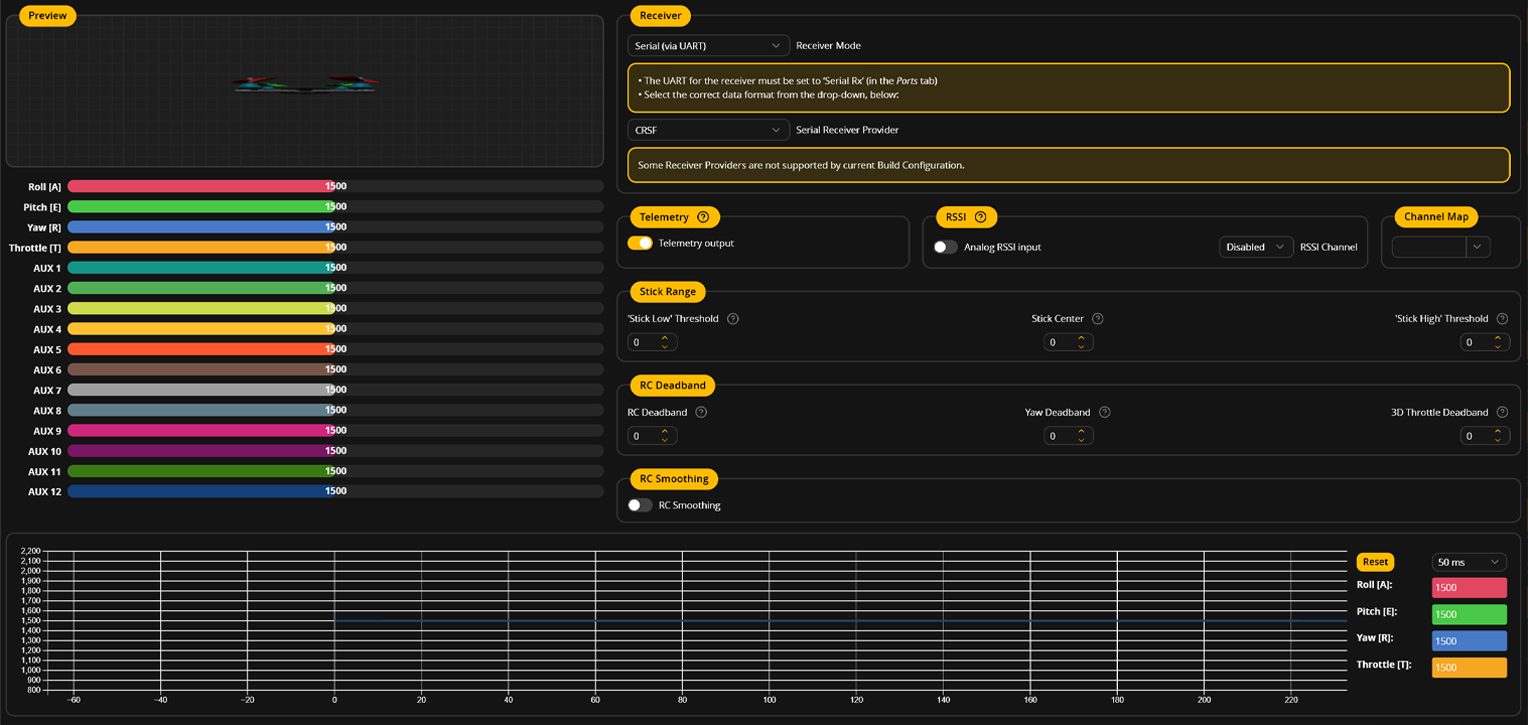
\includegraphics[width=\linewidth]{img/bf-receiver.png}\caption{Receiver}\end{subfigure}\\[2mm]
\begin{subfigure}[b]{0.49\linewidth}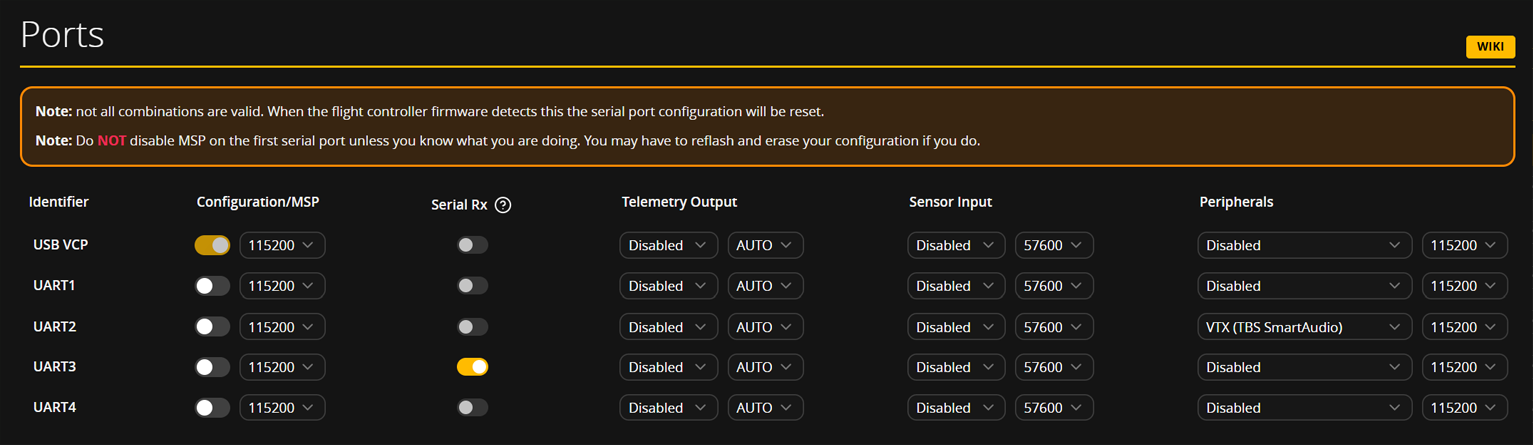
\includegraphics[width=\linewidth]{img/bf-ports.png}\caption{Ports — назначение UART}\end{subfigure}\hfill
\begin{subfigure}[b]{0.49\linewidth}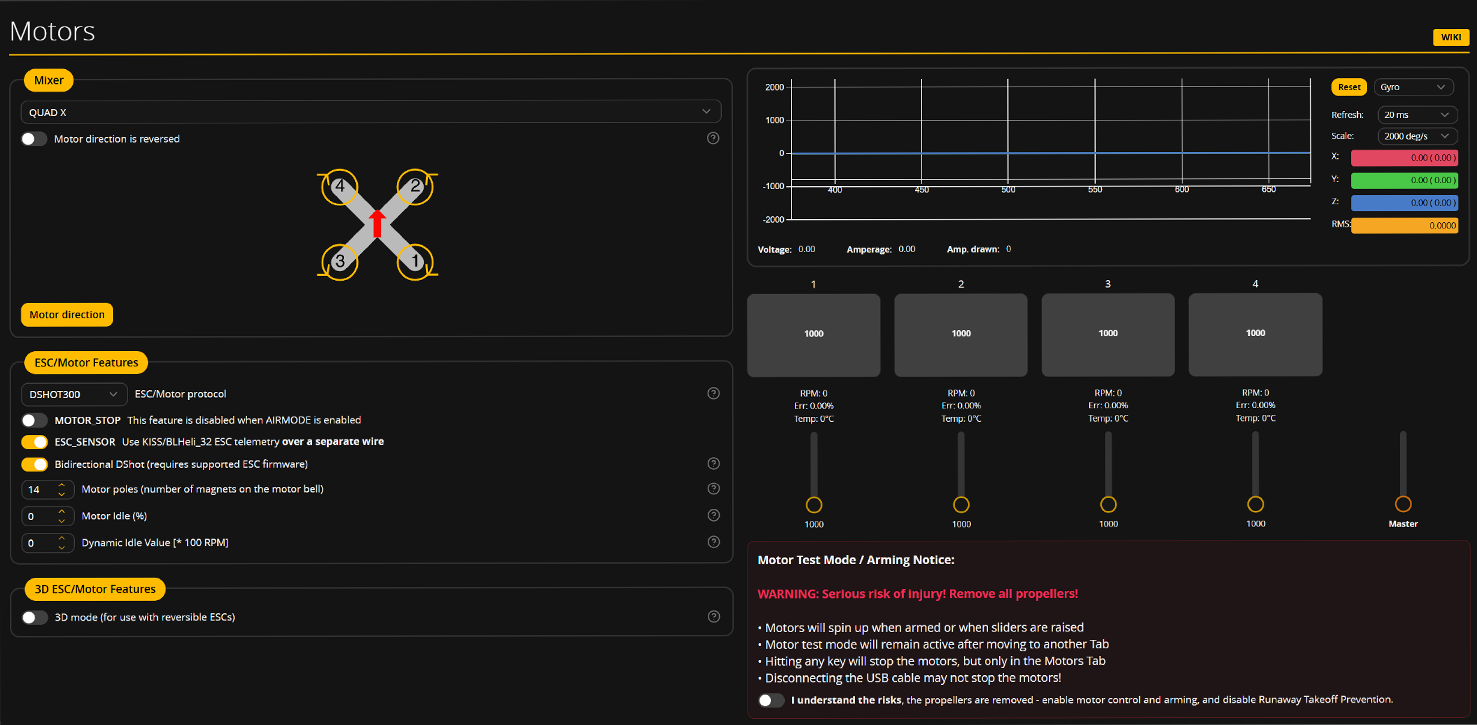
\includegraphics[width=\linewidth]{img/bf-motors.png}\caption{Motors — проверка моторов}\end{subfigure}
\caption{Betaflight Configurator {\color{gray}\scriptsize(скриншоты: документация Betaflight, betaflight.com)}}
\end{figure}

\subsection{INAV}
\begin{itemize}
\item \textbf{Назначение}: навигация. Форк Cleanflight с упором на GPS. Поддерживает мультикоптеры, \textbf{самолёты и летающие крылья}, VTOL, роверы, лодки.
\item Режимы: \term{Position Hold}, \term{Altitude Hold}, \term{RTH} (возврат домой), \term{Waypoint}-миссии (полёт по точкам), Cruise, Loiter, Launch (запуск с руки для самолёта), автопосадка.
\item Программа: \textbf{INAV Configurator} (интерфейс похож на Betaflight) + планировщик миссий, \term{Programming Framework} (логические условия прямо в прошивке), mixer profiles для VTOL.
\item Требует GPS, компас (для коптеров) и барометр. Работает на тех же платах F4/F7/H7, что и Betaflight.
\end{itemize}

\subsection{ArduPilot}
\begin{itemize}
\item \textbf{Назначение}: профессиональный открытый автопилот. Прошивки: \textbf{ArduCopter}, \textbf{ArduPlane} (включая QuadPlane/VTOL), \textbf{Rover}, \textbf{ArduSub} (подводные), \textbf{AntennaTracker}, Blimp.
\item Работает на Pixhawk/Cube, Matek H743 и других H7/F7-платах, а также на Linux (Raspberry Pi, Navio).
\item Протокол \term{MAVLink} — телеметрия и команды. Фильтр Калмана \term{EKF3} для оценки положения.
\item Наземные станции: \textbf{Mission Planner} (Windows), \textbf{QGroundControl} (все ОС и Android), MAVProxy (консоль).
\item Возможности: 20+ режимов (Stabilize, AltHold, Loiter, Auto, RTL, Guided, Land, SmartRTL\ldots), сложные миссии, геозоны, парашют, обход препятствий, скрипты на \textbf{Lua}, компаньон-компьютер (ROS), DroneCAN, резервирование датчиков.
\end{itemize}

\begin{figure}[H]\centering
\begin{subfigure}[b]{0.49\linewidth}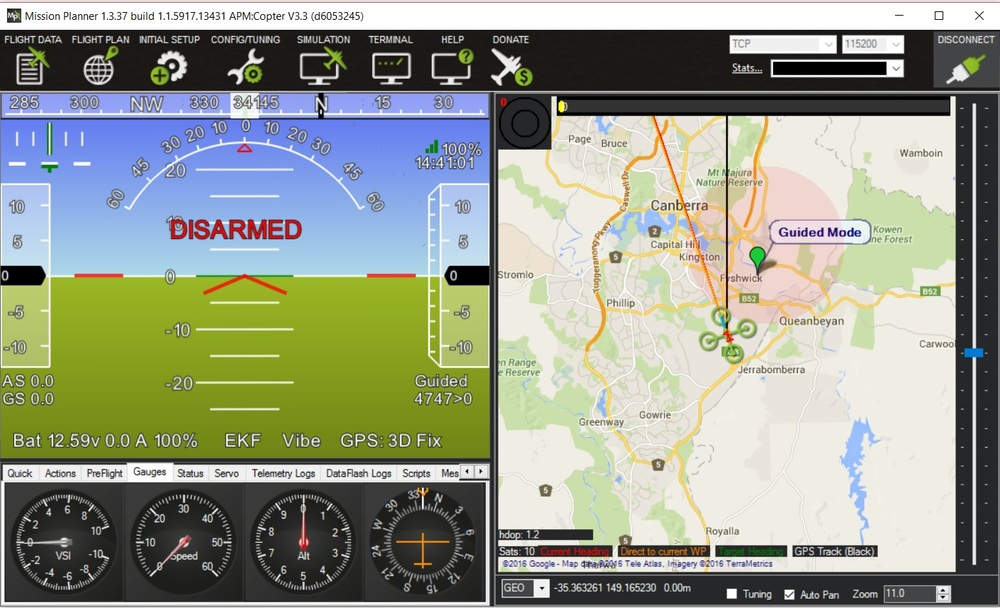
\includegraphics[width=\linewidth]{img/mp-data.jpg}\caption{Flight Data — авиагоризонт и карта}\end{subfigure}\hfill
\begin{subfigure}[b]{0.49\linewidth}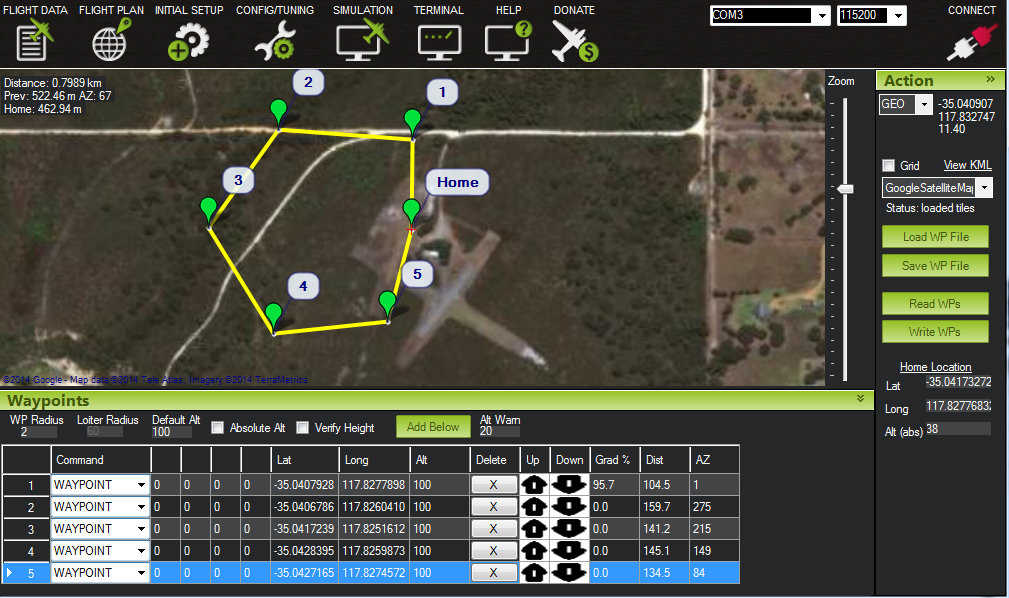
\includegraphics[width=\linewidth]{img/mp-plan.jpg}\caption{Flight Plan — планирование миссии}\end{subfigure}
\caption{Mission Planner для ArduPilot {\color{gray}\scriptsize(скриншоты: ArduPilot Wiki)}}
\end{figure}

\subsection{Сравнение}
\begin{table}[H]\centering\small
\renewcommand{\arraystretch}{1.3}
\begin{tabularx}{\linewidth}{@{}p{28mm} X X X@{}}
\toprule
 & \textbf{Betaflight} & \textbf{INAV} & \textbf{ArduPilot} \\
\midrule
Для чего & FPV, гонки, фристайл & FPV-дальнолёты, самолёты, навигация & Автономные миссии, коммерческие и научные задачи \\
Типы БВС & мультикоптеры & коптеры, самолёты, крылья, VTOL & всё: коптер, самолёт, VTOL, вертолёт, ровер, лодка, подлодка \\
GPS-функции & только GPS Rescue & удержание, RTH, миссии & полный набор + геозоны \\
ПО & Betaflight Configurator & INAV Configurator & Mission Planner, QGroundControl \\
Протокол & MSP & MSP (+ MAVLink телеметрия) & MAVLink \\
Сложность & низкая & средняя & высокая (сотни параметров) \\
Железо & F4/F7/H7 FPV-платы & F4/F7/H7 FPV-платы & Pixhawk, Cube, H7-платы \\
\bottomrule
\end{tabularx}
\caption{Betaflight, INAV, ArduPilot}
\end{table}

\subsection{Вспомогательное ПО}
\begin{itemize}
\item \textbf{ESC Configurator} (веб), \textbf{BLHeliSuite32}, \textbf{AM32 Configurator} — прошивка и настройка регуляторов.
\item \textbf{ExpressLRS Configurator} — прошивка приёмников и модулей ELRS (или через Wi-Fi прямо с устройства).
\item \textbf{EdgeTX / OpenTX} + \textbf{EdgeTX Companion} — прошивка пультов (моделей, микшеров, Lua-скриптов).
\item \textbf{Blackbox Explorer}, \textbf{PID Toolbox} — анализ логов; \textbf{симуляторы}: Liftoff, VelociDrone, Uncrashed, DRL — тренировка без риска.
\end{itemize}

\begin{keybox}[Типичный порядок настройки нового FPV-дрона в Betaflight]
Прошить ПК (Firmware Flasher) $\to$ Setup: калибровка акселерометра $\to$ Ports: включить Serial RX на UART приёмника $\to$ Configuration: протокол ESC (DShot600), ориентация $\to$ Receiver: протокол CRSF, проверить каналы и порядок AETR $\to$ Modes: ARM на тумблере $\to$ Motors: проверить порядок и направление вращения (\textbf{без пропеллеров!}) $\to$ Failsafe $\to$ OSD и VTX $\to$ пробный полёт.
\end{keybox}

\begin{exam}
\begin{enumerate}
\item Какую прошивку выбрать для гоночного дрона, для крыла-дальнолёта, для картографирования по миссии?
\item Что такое режим Acro и чем он отличается от Angle?
\item Что такое MAVLink? Какие наземные станции вы знаете?
\end{enumerate}
\end{exam}
